\tikzsetnextfilename{fbd1}
\begin{center}
   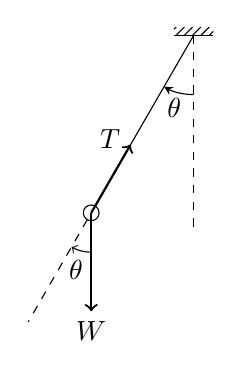
\begin{tikzpicture}

      \def\r{2.5}       % Radius of the string

      \usetikzlibrary{patterns}
% We define a tikz style which defines a fill pattern consisting of lines in the north east direction.
% The draw=none option indicates that we do NOT want any stroke/border around the fill
\tikzstyle{wall}=[fill,pattern=north east lines,minimum width=0.75cm,minimum height=0.3cm, draw=none]


% Define dimensions and angles
\def\hw{0.25}     % Half width of the small wall segment on top

\def\angle{-120}  % Angle of string

\def\br{0.1}      % Radius of bob

\def\ar{0.75}      % Radius of the arc that represents the angle

% NOTE: The macro \r is NOT defined in this file. It must be defined in the calling code before this code is called.


% Define coordinates used in the diagram
\coordinate (bc) at (\angle:\r+\br);          % Center of the bob


% Draw commands
\draw (-\hw, 0) -- (\hw, 0);
\draw [wall] (-\hw,0) rectangle (\hw,0.1);        % Draws a rectangle using the 'wall' pattern giving us the sloped lines

\draw (0,0) -- (\angle:\r);       % string
\draw [dashed] (0,0) -- (0,-\r);  % Dashed line down the middle

\draw (bc) circle [radius=\br];        % The small circle representing the bo;


      % Arc and symbol for the angle at the pivot
      \draw [->,>=stealth] (0, -\ar) arc (-90:\angle:\ar);
      \draw (-105:\ar+0.2) node {$\theta$};

      % Draw the two forces
      \draw [->,thick] (bc) -- ++(0,-1.25) node [below] {$W$};
      \draw [->,thick] (bc) -- ++ (\angle+180:1) node [anchor=south east, yshift=-5] {$T$};

      % Extend string using dashed line to show angle between vector W and the string
      \draw [dashed] (bc) ++ (\angle:\br) -- ++ (\angle:1.5);
      \draw [->] (bc) ++ (0,-0.5) arc (-90:\angle:0.5);
      \draw (bc) ++ (-105:0.75) node {$\theta$};

   \end{tikzpicture}
\end{center}
